\section{Master}
% What responsibilities does M have?
% How is M structured?
% What models does M contain?
% What controllers should M contain, and what should be in these controllers?
% What views does M need?
% How should the web application of M look?

The functionality of Master described in Section~\ref{sec:functionality_distrubution} dictates the structure of \deno{M} to be as shown in Figure~\ref{fig:int_struct_m}. This figure shows three processes; Web, Database, and Daemon. The Database process can be any database engine that can handle transactions, therefore this will not be elaborated further. The Web and Daemon processes will need further explanation, however. \\

\begin{figure}[!ht]
    \centering
    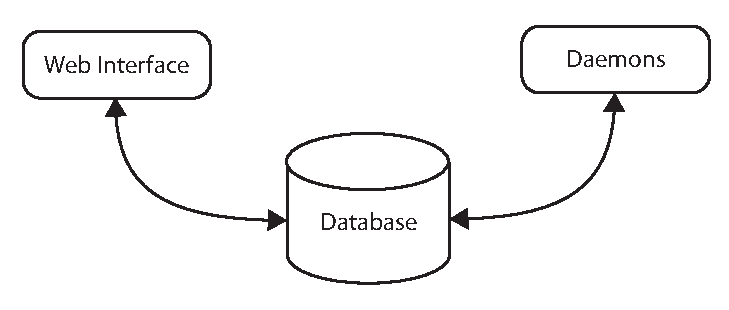
\includegraphics[width=\textwidth]{gfx/master_internal_structure.pdf}
    \caption{Internal structure of Master}
    \label{fig:int_struct_m}
\end{figure}

The web process will be a web server running on an MVC architecture. There are several frameworks in different languages that can used for this, which will be considered in Section~\ref{sec:tools}.

\subsection{Design language}
\fxfatal{Bjarke og Thomas tag stilling}
The design language, which is also known as design vocabulary, is the design guidelines for \projectname{}.
The objects here will have an important role in the systems user interface, and their design language is therefore described here.

\subsubsection{Color scheme}
\begin{figure}[htb]
    \centering
    
\includegraphics[width=\textwidth]{gfx/color_schema.pdf}
    \caption{color schema of \projectname{}.}
    \label{fig:color_schema}
\end{figure}

The color schema seen in \figref{fig:color_schema} shows the colors that are being used in the applications design. \fixme{hvorfor har vi valgt de farver fremfor orange og lyserød?}

\subsubsection{Fonts}
The family of fonts will be: Arial, Helvetica.
These fonts have been selected because they are common both in Windows and Mac and therefore they are browser safe \cite{common_fonts}, meaning that the system will look the same no matter what operating system the user is using.

\subsubsection{Shapes}
All boxes that the user can interact with in the system, will be displayed with rounded corners.
This was done to make the interaction with the boxes as simple and straight forward as possible for the user.

\subsubsection{Layouts}
\begin{figure}[htb]
    \centering
    
\includegraphics[width=\textwidth]{gfx/menu.pdf}
    \caption{The menu of the application, with the control menu point activated.}
    \label{fig:menu_design}
\end{figure}

In \figref{fig:menu_design} the menu of the application is seen.
In the figure, the bullet ``Control'' is active and therefore shown with a grey background color.
All other menues have a black background color and are seperated with white spaces.

\begin{figure}[htb]
    \centering
    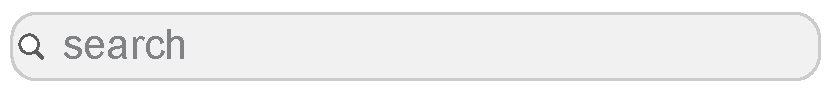
\includegraphics[width=\textwidth]{gfx/search.pdf}
    \caption{Search bar of the application}
    \label{fig:search_bar_design}
\end{figure}

In \figref{fig:search_bar_design} the search bar of the application is seen.
The ``search'' text will disappear when the bare is clicked, and if the user types anything this will be shown in the search bar instead.

\begin{figure}[htb]
    \centering
    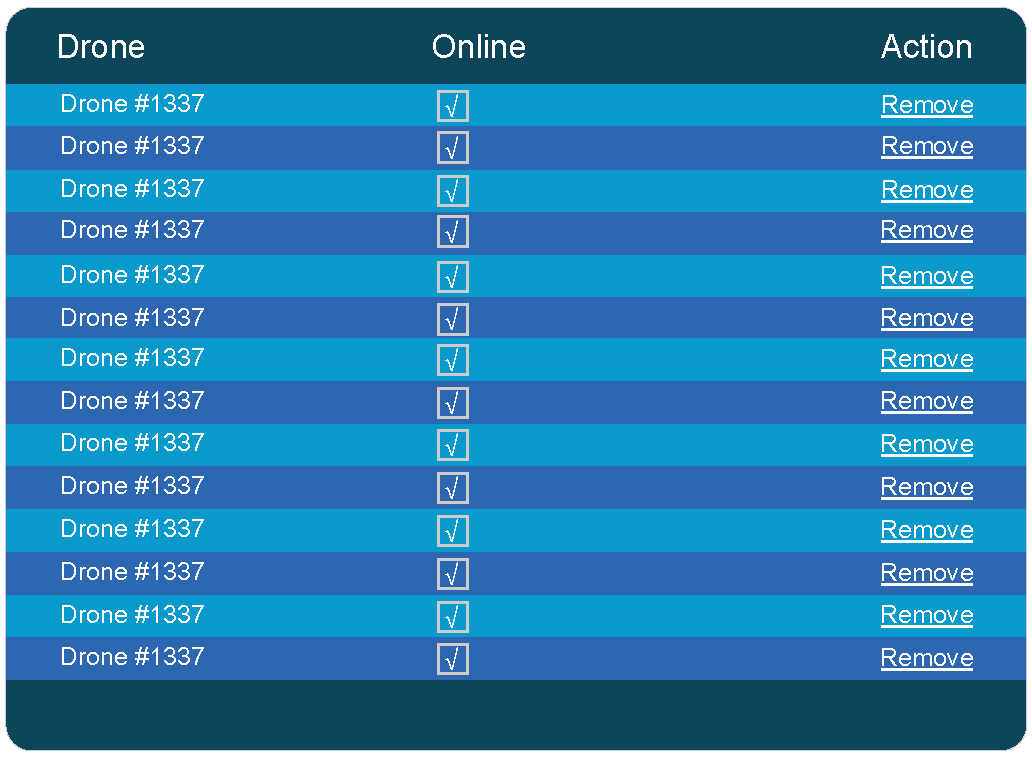
\includegraphics[width=\textwidth]{gfx/table.pdf}
    \caption{Table design for the application.}
    \label{fig:table_design}
\end{figure}
In \figref{fig:table_design} the general design for tables of the application is seen.
Odd rows will be light blue and even rows will be blue.

\begin{figure}[htb]
    \centering
    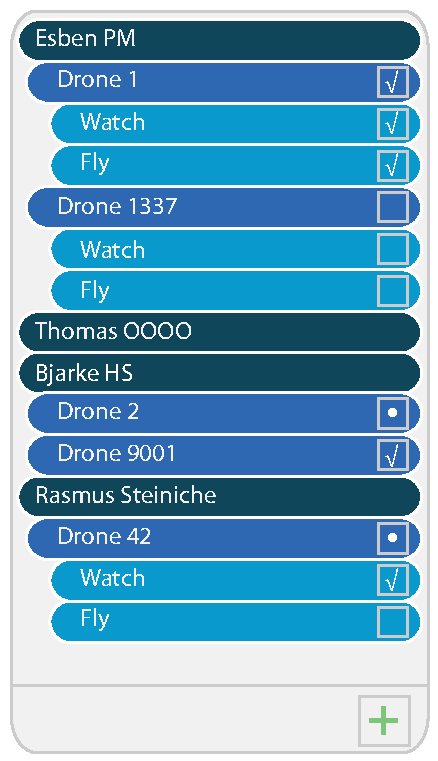
\includegraphics[scale=1.0]{gfx/list.pdf}
    \caption{List design for the application.}
    \label{fig:list_design}
\end{figure}
The list design shown in \figref{fig:list_design} is designed to show a tree-structured list.
This example shows the relationship between drones, privileges and users, where it is possible to activate different privileges on a given drone for a given user.
Each type of element (user, drone and privilege) as separate colors to make it easier to get an overview of the list. \\

Each privilege can have three different marks:

\begin{itemize}
    \item Not marked
    \item Dotted
    \item Ticked
\end{itemize}

If no privileges are marked, as seen with ``Drone 1337'', the user has no privileges to access this drone.
If a box is dotted, as seen with ``Drone 42'', the user s some privileges for this drone.
And finally, if a box is ticked, as seen with ``Drone 1'', the user has all privileges for this drone.

\begin{figure}[htb]
    \centering
    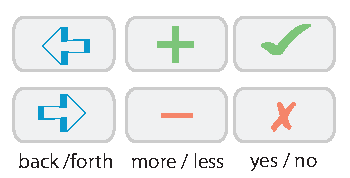
\includegraphics[scale=1.0]{gfx/button.pdf}
    \caption{Button design for the application.}
    \label{fig:button_design}
\end{figure}

The buttons used in \projectname{} has also gotten their own design to match the rest of the view.
There are six buttons:
Back, Forth, More, Less, Yes, \& No.
These will be used in the user interface where appropriate.
They do not carry any functionality, but are merely standard buttons with nicer looks.
